\documentclass[12pt,aspectratio=169]{beamer}
\usetheme{metropolis}
\setbeamersize{text margin left=.5cm,text margin right=.5cm}
%\usefonttheme{professionalfonts}
\usepackage[lf]{carlito}
\usepackage{tikz}
\usepackage{mathpazo}
\usepackage{bm}
\usepackage{xcolor,colortbl}
\usepackage{siunitx}

\sisetup{
  inter-unit-product=\cdot,
  per-mode=symbol
}
\tikzset{>=latex}

\setlength{\parskip}{0pt}
\renewcommand{\baselinestretch}{1}


\title{Topic 10: Thermodynamics}
\subtitle{Advanced Placement Physics 2}
\author[TML]{Dr.\ Timothy Leung}
\institute{Olympiads School}
\date{\today}

\newcommand{\pic}[2]{
  \begin{center}
    \includegraphics[width=#1\textwidth]{#2}
  \end{center}
}
\newcommand{\eq}[2]{
  \vspace{#1}{\Large
    \begin{displaymath}
      #2
    \end{displaymath}
  }
}

\begin{document}

\begin{frame}
  \maketitle
\end{frame}



\begin{frame}{Kinetic Theory of Gases}
  We begin the study of the thermodynamics of ideal gases using these
  assumptions:
  \begin{enumerate}
  \item The gas consists of a large number of identical molecules that are in
    high-speed random motion
  \item Molecular motion and interaction obey Newtonian laws of motion
  \item Collision between molecules and with the walls of the container are
    \emph{elastic}
  \item Molecules are separated, on average, by distances that are large
    compared to their diameters (i.e.\ the space occupied by the molecules are
    small compared to the space occupied by the gas as a whole)
  \item The only forces that the molecules experience are \emph{contact} forces
    (i.e.\ no gravitational, electrostatic etc forces on each other except when
    they collide)
  \end{enumerate}
\end{frame}



\begin{frame}{Properties of a Gas}
  \begin{itemize}
  \item\textbf{Volume} is the space occupied by the gas, with a unit of
    \textbf{cubic meter} (\si{\metre\cubed})
  \item\textbf{Pressure} is the force $F$ that a gas exerts on the container,
    divided by the surface area of the container $A$ when the molecules collide
    with it:
    \begin{displaymath}
        P=\frac FA
    \end{displaymath}
    \begin{itemize}
    \item\vspace{-.2in}Unit of pressure: \textbf{pascal} (\si{\pascal})
    \item At thermal equilibrium, pressure is evenly distributed in the gas
    \end{itemize}
  \item\textbf{Temperature} is a measure of the average kinetic energy of the
    gases.
    \begin{itemize}
    \item It measures how ``hot'' an object is
    \item SI Unit of temperature: \textbf{kelvin} (\si{\kelvin})
    \end{itemize}
  \end{itemize}
\end{frame}


\section{Thermodynamic Temperature}

\begin{frame}{Thermodynamic Temperature}
  William Thomson (Lord Kelvin) and James Joule discovered that when a gas is
  heated or cooled at \emph{constant volume}, there is a \emph{linear}
  relationship between pressure and temperature:
  \begin{center}
    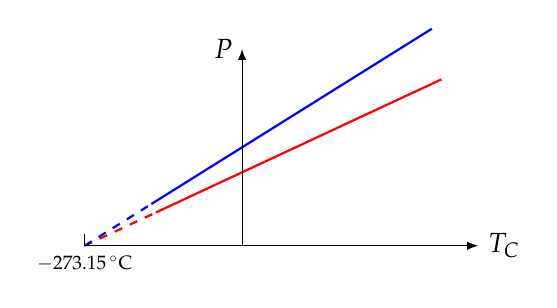
\begin{tikzpicture}
      \begin{scope}[rotate=25]
        \draw[thick,red,dashed](0,0)--(1,0);
        \draw[thick,red](1,0)--(5,0);
      \end{scope}
      \begin{scope}[rotate=32]
        \draw[thick,blue,dashed](0,0)--(1,0);
        \draw[thick,blue](1,0)--(5.2,0);
      \end{scope}
      \draw[->](0,0)--(5,0) node[right]{$T_C$};
      \draw(0,0)--(0,.15) node[pos=0,below]{\scriptsize\SI{-273.15}{\celsius}};
      \draw[->](2,0)--(2,2.5) node[left]{$P$};
    \end{tikzpicture}
  \end{center}
  Regardless of the type of gas, amount of gas, or the volume of gas, pressure
  is always zero at \SI{-273.15}{\celsius}. Since pressure cannot be negative;
  no temperature exists below that value.
\end{frame}



\begin{frame}{Thermodynamic Temperature}
  The \textbf{thermodynamic temperature}\footnote{or \textbf{absolute
      temperature}} $T$
  is obtained by shifting the ``null point'' (where temperature is zero) from
  the Celsius temperature $T_C$.
  
  \eq{-.2in}{
    \boxed{T = T_C + 273.15}
  }
  \begin{itemize}
  \item\vspace{-.1in}A temperature of \SI0{\kelvin} is called
    \textbf{absolute zero}\footnote{Absolute zero is impossible to obtain
      because of quantum-mechanic effects}
  \item This temperature scale is consistent with the physical and
    thermodynamic properties of gases
  \item Note: the temperature \emph{change} of \SI1{\kelvin} is the same as
    \SI1{\celsius}, i.e.:

    \eq{-.25in}{
      \Delta T=\Delta T_C
    }
  \end{itemize}
  \vspace{.25in}
\end{frame}
  


%\begin{frame}{Relationship Between Temperature and Pressure}
%  The relationship between absolute temperature $T$ and pressure $P$
%  of a gas at constant volume is defined using its triple point:
%
%  \eq{-.1in}{
%    T=\frac{T_\text{tp}}{P_\text{tp}}P
%  }
%
%  \textbf{Triple point} is a combination of pressure and temperature where all
%  phases of a substance (solid, liquid and vapour) may coexist in thermal
%  equilibrium.
%  \begin{itemize}
%  \item The triple point temperature for water is at
%    $T_\text{tp}=\SI{273.16}{\kelvin}$, or $\SI{0.01}{\celsius}$
%  \item Triple point pressure for water is $P_\text{tp}=\SI{611.2}{\pascal}$
%  \end{itemize}
%\end{frame}
%
%
%
%\begin{frame}{Thermal Expansion}
%  When temperature $T$ of an object with length $L$ increases, the object
%  \emph{usually} expands. The \emph{thermal strain} ($\Delta L/L$) is
%  proportional the change in temperature ($\Delta T$) by the \textbf{coefficient
%    of linear thermal expansion} ($\alpha$):
%  
%  \eq{-.15in}{
%    \boxed{\frac{\Delta L}{L} =\alpha\Delta T}
%  }
%  \begin{center}
%    \begin{tabular}{l|c|c}
%      \rowcolor{pink}
%      \textbf{Quantity} & \textbf{Symbol} & \textbf{SI Unit} \\ \hline
%      Length      & $L$  & \si{\metre}  \\
%      Temperature & $T$  & \si{\kelvin} \\
%      Coefficient of linear expansion & $\alpha$ & \si{\per\kelvin}
%    \end{tabular}
%  \end{center}
%  $\alpha$ is independent of pressure for solids and liquids, but may vary
%  with $T$.
%\end{frame}
%
%
%
%\begin{frame}{Thermal Expansion}
%  There is also a similar expression for \textbf{coefficient of volume
%    expansion}:
%  
%  \eq{-.15in}{
%    \boxed{\frac{\Delta V}V=\beta\Delta T}
%  }
%
%  $\beta$ is also independent of pressure for solids and liquids,
%  but may vary with $T$.
%  \begin{center}
%    \begin{tabular}{l|c|c}
%      \rowcolor{pink}
%      \textbf{Quantity} & \textbf{Symbol} & \textbf{SI Unit} \\ \hline
%      Volume      & $V$  & \si{\metre\cubed} \\
%      Temperature & $T$  & \si{\kelvin} \\
%      Coefficient of volume expansion & $\beta$ & \si{\per\kelvin} \\
%    \end{tabular}
%  \end{center}
%  Careful application of calculus will show that for isotropic material (where
%  $\alpha$ is the same in all direction)
%
%  \eq{-.4in}{
%    \beta = 3\alpha
%  }
%\end{frame}



\section{Ideal Gas Law}

\begin{frame}{Ideal Gas Law for Low-Density Gases}
  Robert Boyle (1627-1691) discovered that, when a gas is allowed to expand or
  compress at \emph{constant temperature}, the product of pressure $P$ and $V$
  remain constant (\textbf{Boyle's law}):

  \eq{-.2in}{
    PV=\text{constant}
 }

  \vspace{-.1in}From the previous discussion on temperature scale, we also know
  that at \emph{constant volume}, (thermodynamic) temperature is proportional to
  pressure. Combining the two discoveries yields this equation:

  \eq{-.25in}{
    PV=CT
  }

  \vspace{-.2in}where ``C'' is some constant to be determined.
\end{frame}



\begin{frame}{Ideal Gas Law}
  Thought experiment:
  \begin{itemize}
  \item Two identical containers with the same volume $V$, same amount of same
    kind of gas, at same pressure $P$ and same temperature $T$
  \item When the containers are combined and the molecules are free to move,
    $P$ and $T$ remain the same, but volume and the number of molecules are
    both increased by factor of 2
  \end{itemize}
  Therefore $C$ must scale with the number of molecules of gas $N$, which
  modifies the equation to this, the \textbf{ideal gas law}:

  \eq{-.25in}{
    \boxed{PV=Nk_BT}
  }

  \vspace{-.15in}The constant $k_B=\SI{1.381e-23}{\joule\per\kelvin}$ is called
  \textbf{Boltzmann's constant}. It is found experimentally to have the same
  value for any kind or amount of gas.
\end{frame}



\begin{frame}{Ideal Gas Law}
  The ideal gas law is often expressed in a different form in chemistry
  courses:  

  \eq{-.25in}{
    \boxed{PV=nRT}
  }

  \vspace{-.2in}where:
  \begin{itemize}
  \item $n=N/N_A$ is the number of moles of the gas
  \item $R=kN_A=\SI{8.314}{\kilo\gram/\mol.\kelvin}$ is the
    \textbf{universal gas constant}, and
  \item $N_A=\num{6.022e23}$ is \textbf{Avagadro's number}, which is the number
    of molecules in one mole
  \end{itemize}

  \vspace{.1in}The ideal gas law is an \textbf{equation of state}, because it
  relates all the quantities that define the \emph{state} of a gas: pressure
  $P$, volume $V$ and temperature $T$.
\end{frame}



\section{Maxwell-Boltzmann Distribution}

\begin{frame}{Maxwell-Boltzmann Distribution}
  As gas molecules collide elastically with each other inside the
  container\footnote{Recall the discussion on elastic collision from earlier in
    the course}:
  \begin{itemize}
  \item Some molecules \emph{gain} kinetic energy (therefore moving faster),
    while
  \item Some molecules \emph{lose} kinetic energy (therefore moving slower)
  \item Individual collisions are random occurances (determined by statistical
    probabilities), but
  \item The overall behavior of the molecules at thermal equilibrium is very
    predictable
  \end{itemize}
\end{frame}



\begin{frame}{Maxwell-Boltzmann Distribution}
  The distribution of particle velocities for a gas in a container is
  pproximated by a probability distribution function called the
  \textbf{Maxwell-Boltzmann distribution}:

  \eq{-.2in}{
    f(v)=4\pi\left[\frac{m}{2\pi k_BT}\right]^{\frac32}v^2
    \exp\left[-\frac{mv^2}{2k_BT}\right]
  }

  \begin{center}
    \begin{tabular}{l|c|c}
      \rowcolor{pink}
      \textbf{Quantity} & \textbf{Symbol} & \textbf{SI Unit} \\ \hline
      Maxwell-Boltzmann dist.\ function & $f(v)$ &\si{\second\per\metre}\\
      Molecular mass            & $m$        & \si{\kilo\gram} \\
      Particle speed            & $v$        & \si{\metre\per\second} \\
      Thermodynamic temperature & $T$        & \si{\kelvin} \\
      Boltzmann's constant      & $k_B$      & \si{\joule\per\kelvin}
    \end{tabular}
  \end{center}
  AP Physics 2 is not too concerned with the (difficult) mathematics,
  but rather, the overall concept.
\end{frame}



\begin{frame}{Maxwell-Boltzmann Distribution}
  \vspace{.15in}\begin{columns}
    \column{.45\textwidth}
    \pic{1.05}{maxwell-boltzmann}
    
    \column{.55\textwidth}
    \begin{itemize}
    \item The area under the distribution curve is 1 (all probabilites sums to
      \SI{100}{\percent})
    \item The peak of the distribution shifts to higher speeds as $T$ increases
    \item The peak, which represents the most-probable speed $v_\text{prob}$,
      is lower at higher temperatures.
    \end{itemize}
  \end{columns}
  \vspace{.2in}There are three particles speeds that are important: the
  most-probable speed $v_\text{prob}$, the mean (average) speed
  $\langle v \rangle$ and the root-mean-square speed $v_\text{rms}$.
\end{frame}



\begin{frame}{Maxwell-Boltzmann Distribution}
  \vspace{.15in}\begin{columns}
    \column{.48\textwidth}
    \pic{1}{speed-distribution}
    
    \column{.52\textwidth}
    The \textbf{most probable speed} $v_\text{prob}$ is the peak of the
    distribution function, where the speed is maximum (i.e.\ the mode of the
    function):

      \eq{-.2in}{
        v_\text{prob}=\sqrt{\frac{2k_BT}m}
      }
  \end{columns}
  \vspace{.2in}It is obtained through using basic (albeit not necessarily
  simple) calculus.\footnote{Finding the derivative of $f(v)$ using chain rule
    and solving for $f'(v)=0$}
  \vspace{.3in}
\end{frame}



\begin{frame}{Maxwell-Boltzmann Distribution}
  The \textbf{mean speed} $\langle v \rangle$ (or \textbf{average speed}) is
  calculated using the definition of an average using the weighted sum over $N$
  particles\footnote{The proper calculus notation is the integral
    $\int_0^\infty vf(v)dv$}:
  \begin{displaymath}
    \langle v\rangle =\frac{v_1+v_2+\cdots+v_N}N
  \end{displaymath}
  \begin{columns}
    \column{.48\textwidth}
    \pic{1}{speed-distribution}
    
    \column{.52\textwidth}
    This average speed is found to be:

      \eq{-.2in}{
        \langle v \rangle =\sqrt{\frac{8k_BT}{\pi m}}
      }
  \end{columns}
  \vspace{.15in}
\end{frame}



\begin{frame}{Root Mean Square Speed}
  When studying the behavior of gases, the quantity of interest is often the
  average \emph{kinetic energy} of the molecules $\langle K\rangle$, which
  scales with $v^2$. The weighted average of kinetic energy:\footnote{Again,
    the proper calculus notation is the integral $\int_0^\infty v^2f(v)dv$.}
  \begin{displaymath}
    \langle K\rangle=\frac{\frac12mv_1+\cdots+\frac12mv_N^2}{N}
    =\frac12m
    \underbrace{\left[\frac{v_1^2+v_2^2+\cdots+v_N^2}N\right]}_{v_\text{rms}^2}
  \end{displaymath}
  The speed that gives the average kinetic energy is called the \textbf{root
    mean square speed} $v_\text{rms}$:

  \eq{-.3in}{
    v_\text{rms}=\sqrt{\frac{3k_BT}{m}}
  }
  \vspace{.2in}
\end{frame}



\begin{frame}{Average Kinetic Energy of a Gas}
  From the expression of $v_\text{rms}$, and relating to the average kinetic
  energy, it is easy to show that:
  
  \eq{-.2in}{
    \langle K \rangle=\frac12v_\text{rms}^2=
    \frac12\left(\sqrt{\frac{3k_BT}m}\right)^2
    \quad\rightarrow\quad
    \boxed{\langle K\rangle=\frac32k_BT}
  }

  i.e.\ thermodynamic temperature represents the average kinetic energy. If the
  number of gas molecules is known (which is usually not the case), then the
  \emph{total} kinetic energy is just:

  \eq{-.2in}{
    K=N\langle K\rangle=\frac32Nk_BT
  }
\end{frame}



\begin{frame}{$P$-$V$ Diagram}
  Thermodynamic processes is usually plotted on a ``$P$-$V$ diagram''.
  \begin{columns}
    \column{.35\textwidth}
    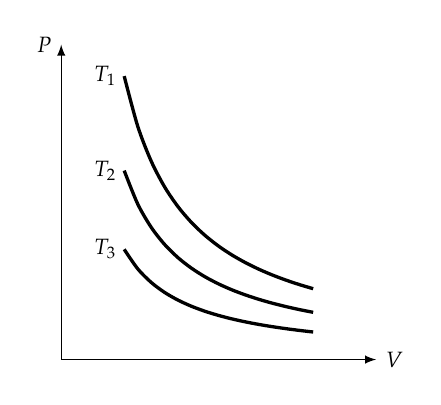
\begin{tikzpicture}[scale=.8]
      \draw[->](0,0)--(5,0) node[right]{\footnotesize $V$};
      \draw[->](0,0)--(0,5) node[left]{\footnotesize $P$};
      \draw[smooth,samples=15,domain=1:4,very thick] plot({\x},{1.75/\x});
      \draw[smooth,samples=15,domain=1:4,very thick] plot({\x},{3/\x});
      \draw[smooth,samples=15,domain=1:4,very thick] plot({\x},{4.5/\x});
      \node (t1) at (.7,1.75){\footnotesize $T_3$};
      \node (t1) at (.7,3)   {\footnotesize $T_2$};
      \node (t1) at (.7,4.5) {\footnotesize $T_1$};
    \end{tikzpicture}

    \column{.65\textwidth}
    \begin{itemize}
    \item Under constant temperature, the relationship between pressure and
      volume is a hyperbolic curve.
    \item Each line is called an \textbf{isotherm}; it represents a different
      constant temperature
    \item $T_3>T_2>T_1$
    \end{itemize}
  \end{columns}
  
  \vspace{.2in}{\footnotesize\textbf{Note:} Aside from $P$-$V$ diagrams, there
    are many similar diagrams in thermodynamics. \par}
\end{frame}



\begin{frame}{Real Gases}
  Most gases behave like ideal gas at most ordinary pressures, but the
  equation breaks down when the density of gas is high and molecules are not
  far apart:
  \begin{itemize}
  \item pressure is sufficiently high
  \item temperature is low
  \end{itemize}
  In these situations the \textbf{van der Waal equation} provides a more
  accurate description of the behavior of real gases:

  \eq{-.2in}{
    \boxed{\left(P+\frac{an^2}{V^2}\right)(V-bn)=nRT}
  }

  \begin{itemize}
  \item The term $an^2/V^2$ is from the attraction of the gas molecules to each
    other
  \item The term $b$ is approximately the volume occupied by one mole of the gas
  \end{itemize}
\end{frame}



\begin{frame}{Real Substances}
  Neither the ideal gas law nor the van der Waal equation capture the exact
  relationship between pressure and volume, because neither accounts for phase
  changes. The $P$-$V$ diagram of a real substance is like this:
  \pic{.35}{realsubstance}
\end{frame}



\begin{frame}{Phase Diagrams}
  The phase diagram plots pressure against temperature to show when the
  different phases of matter exist. For water:
  \pic{.4}{10-figure-31}
  \begin{itemize}
  \item\vspace{-.1in} At \textbf{triple point} $B$, all three phases of matter
    can exist in equilibrium
  \item At \textbf{critical point} $C$, liquid and vapour phases are
    indistinguishable, and the gas laws can model their behavior
  \end{itemize}
\end{frame}



\begin{frame}{First Law of Thermodynamics}
  In the \textbf{first law of thermodynamics}, the change in internal energy of
  a thermodynamic system ($\Delta U$) is the difference between the heat added
  into the system and the sum of the work ($W$) \emph{by} the
  system\footnote{\textbf{VERY IMPORTANT NOTE:} Often the equation is written
    as $\Delta U=Q+W$, where $W$ is the work done \emph{to} the system. Since
    both conventions are commonly use, you must be very careful.}:
  
  \eq{-.2in}{
    \boxed{\Delta U=Q-W}
  }
  \begin{center}
    \begin{tabular}{l|c|c}
      \rowcolor{pink}
      \textbf{Quantity} & \textbf{Symbol} & \textbf{SI Unit} \\ \hline
      Change in internal energy of a system & $\Delta U$ & \si{\joule} \\
      Work done \emph{by} the system & $W$               & \si{\joule} \\
      Heat into the system           & $Q$               & \si{\joule}
    \end{tabular}
  \end{center}
\end{frame}


\begin{frame}{First Law of Thermodynamics}
  Internal energy $U$ is the total kinetic \& potential energies of the
  molecules. It is proportional to thermodynamic temperature.

  \eq{-.25in}{
    \boxed{\Delta\textcolor{red}{U}=Q-W}
  }

  \vspace{-.1in}For monatomic gases and ideal gas: there are 3 degrees of
  translational freedom, therefore the internal energy is the total kinetic
  energy, shown a few slides ago:

  \eq{-.25in}{
    U=\frac32Nk_BT
  }

  For diatomic gases, there are 3 degrees of translational freedom and 2
  degrees of rotational freedom:

    \eq{-.32in}{
      U=\frac52Nk_BT
    }
\end{frame}



\begin{frame}{First Law of Thermodynamics}
  \eq{-.2in}{
    \boxed{\Delta\textcolor{red}{U}=Q-W}
  }

  For solids, there are 3 degrees of elastic compression freedom, therefore the
  internal energy is

  \eq{-.3in}{
    U=3Nk_BT
  }

  Note that internal energy does not include:
  \begin{itemize}
  \item The bulk kinetic energy of the system, i.e.\ if the entire container
    of gas moves at speed $v$
  \item The potential energies caused by an external force field (e.g.\
    gravitational, electric, magnetic)
  \end{itemize}
\end{frame}



\begin{frame}{First Law of Thermodynamics}
  \textbf{Heat} \textcolor{blue}{$Q$} is the spontaneous transfer of energy
  \emph{into} the system, through conduction, convection and radiation.

  \eq{-.2in}{
    \boxed{\Delta U=\textcolor{blue}{Q}-W}
  }
  \begin{itemize}
  \item\vspace{-.2in} Heat transfer $Q$ is:
    \begin{itemize}
    \item $+$ if thermal heat is added to the system
    \item $-$ if thermal heat leaves the system
    \end{itemize}
  \item The net flow of energy is always from the higher temperature to low
    temperature
  \item Two objects are in thermal equilibrium if the temperatures are the same
  \end{itemize}
\end{frame}
%    For conduction, the rate of heat transfer $\Delta Q/\Delta t$ (aka ``thermal
%    current'') is given by:
%
%    \eq{-.2in}{
%      \boxed{H=\frac{\Delta Q}{\Delta t}=kA\frac{\Delta T}{\Delta x}}
%    }
%
%    \vspace{-.15in}where $k$ is the thermal conductivity of the material
%
 %   \column{.3\textwidth}
 %   \pic{1}{conduct}
 % \end{columns}


\begin{frame}{Heat Required for a Temperature Change}
  Heat $Q$ required to change the temperature $\Delta T$ is defined as:
  
  \eq{-.2in}{
    \boxed{Q = mc\Delta T}
  }
  \begin{center}
    \begin{tabular}{l|c|c}
      \rowcolor{pink}
      \textbf{Quantity}      & \textbf{Symbol} & \textbf{SI Unit} \\ \hline
      Amount of heat transferred  & $Q$ & \si{\joule} \\
      Mass                        & $m$ & \si{\kilo\gram} \\
      Specific heat capacity      & $c$ & \si{J/kg.K}\\
      Temperature change          & $\Delta T$ & \si{\kelvin}
    \end{tabular}
  \end{center}
  %The \textbf{specific heat capacity} is the energy required to raise the
  %temperature of \SI{1}{\kilo\gram} of a substance by \SI{1}{\kelvin}.
\end{frame}



\begin{frame}{Specific Heat Capacity}
  \begin{columns}
    \column{.55\textwidth}
    \textbf{Specific heat capacity} $c$ is the amount of energy needed to raise
    \SI1{\kilo\gram} of a substance by \SI1{\kelvin}. For gases, $c$ is either
    measured at constant volume or pressure
    \begin{itemize}
    \item\textbf{Constant volume} $c_v$: no work is done; all the heat transfer
      goes to changing the temperature
    \item\textbf{Constant pressure} $c_p$: work $P\Delta V$ is done at constant
      pressure while temperature also changes
    \end{itemize}

    \column{.45\textwidth}
    \begin{tabular}{|l|r|}
      \hline
      \rowcolor{pink}
      \textbf{Substance} & $c$ (\si{J/kg.K}) \\
      \hline
      ethyl alcohol & $2450$ \\
      glycerine     & $2410$ \\
      mercury       & $139$ \\
      water (at \SI{15}{\celsius}) & $4186$ \\
      \hline
      aluminum & $900$ \\
      copper   & $387$ \\
      glass    & $840$ \\
      human body (\SI{37}{\celsius}) & $3500$ \\
      ice (\SI{-15}{\celsius})       & $2000$ \\
      steel    & $452$ \\
      lead     & $128$ \\
      silver   & $235$ \\
      \hline
    \end{tabular}
  \end{columns}
\end{frame}


\begin{frame}{First Law of Thermodynamics}
  \textcolor{green!80!black}{$W$} is the mechanical work\footnote{The full
    definition in calculus form is $W=\int PdV$ (i.e.\ pressure times change in
    volume) which is derived from the definition of mechanical work:
    $W=\int\bm{F}\cdot d\bm{x}$ (force times distance).} done \emph{by}
  the system to the surrounding.

  \eq{-.2in}{
    \boxed{
      \Delta U=Q-\textcolor{green!80!black}{W}
    }
  }
  \begin{itemize}
  \item Work is done iff\footnote{``if and only if''} the volume changes
  \item At constant pressure:

    \eq{-.3in}{
      W=P\Delta V
    }
  \item $+$ done \emph{by} the system, e.g.\ using steam pressure to push a
    piston or shaft
  \item $-$ done \emph{to} the system, e.g.\ pushing a piston to compress gas
    in an engine
  \end{itemize}
  \vspace{.4in}
\end{frame}




\begin{frame}{Work Done By a Gas}
  On the $P$-$V$ diagram, $W$ is the area under the curve.
  \begin{itemize}
  \item $W$ is $+$ (\emph{by} the system) if the path moves right
  \item $W$ is $-$ (\emph{to} the system) if the path moves left
  \end{itemize}
  In the example below, the gas is changed from points $1$ to $2$, but the work
  done is different.
  \begin{center}
    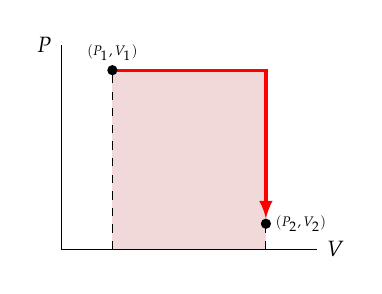
\begin{tikzpicture}[scale=.65]
      \fill[pink!80!gray!50](1,0) rectangle(4,3.5);
      \draw[dashed](1,0)--(1,3.5);
      \draw[dashed](4,0)--(4,.5);
      \draw(0,0)--(5,0) node[right]{\footnotesize $V$};
      \draw(0,0)--(0,4) node[left]{\footnotesize $P$};
      \draw[very thick,->,red](1,3.5)--(4,3.5)--(4,.6);
      \fill(1,3.5) circle(.1) node[above]{\tiny $(P_1,V_1)$};
      \fill(4,.5) circle(.1)  node[right]{\tiny $(P_2,V_2)$};
    \end{tikzpicture}
    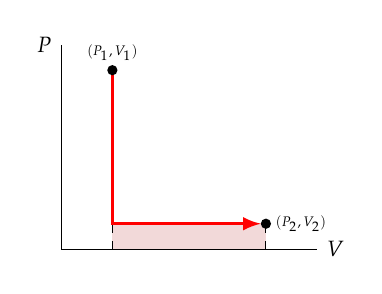
\begin{tikzpicture}[scale=.65]
      \fill[pink!80!gray!50](1,0) rectangle(4,.5);
      \draw[dashed](1,0)--(1,3.5);
      \draw[dashed](4,0)--(4,.5);
      \draw(0,0)--(5,0) node[right]{\footnotesize $V$};
      \draw(0,0)--(0,4) node[left]{\footnotesize $P$};
      \draw[very thick,->,red](1,3.5)--(1,.5)--(3.9,.5);
      \fill(1,3.5) circle(.1) node[above]{\tiny $(P_1,V_1)$};
      \fill(4,.5) circle(.1)  node[right]{\tiny $(P_2,V_2)$};
    \end{tikzpicture}
    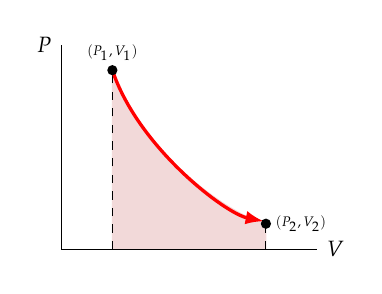
\begin{tikzpicture}[scale=.65]
      \draw[fill=pink!80!gray!50,draw=pink!80!gray!50]
      (1,0)--(1,3.5)..controls(1.5,2) and (3.2,.7)..(4,.5)--(4,0)--cycle;
      \draw[dashed](1,0)--(1,3.5);
      \draw[dashed](4,0)--(4,.5);
      \draw(0,0)--(5,0) node[right]{\footnotesize $V$};
      \draw(0,0)--(0,4) node[left]{\footnotesize $P$};
      \draw[very thick,->,red](1,3.5)..controls(1.5,2) and (3.2,.7)..(3.95,.55);
      \fill(1,3.5) circle(.1) node[above]{\tiny $(P_1,V_1)$};
      \fill(4,.5) circle(.1)  node[right]{\tiny $(P_2,V_2)$};
    \end{tikzpicture}
  \end{center}
  The fact that $W$ is \emph{path dependent} means that the pressure force
  $F=P\cdot A$ is non-conservative.
\end{frame}



\begin{frame}{Quasi-Static Processes}
  A \textbf{quasi-static process} is a thermodynamic process that happens
  slowly enough for the system to remain in internal equilibrium. We are
  concerned with four of these processes:
  \begin{itemize}
  \item\textbf{Isobaric process} - constant pressure
  \item\textbf{Isochoric process} - constant volume
  \item\textbf{Isothermal process} - constant temperature
  \item\textbf{Adiabatic process} - ``isolated'', no heat exchanged with
    surrounding
  \end{itemize}
\end{frame}



\begin{frame}{Quasi-Static Processes}
  \begin{center}
    \begin{tikzpicture}[scale=.6]
      \draw(0,0)--(5,0) node[right]{\footnotesize $V$}
      node[midway,below]{Isobaric};
      \draw(0,0)--(0,4) node[left]{\footnotesize $P$};
      \draw[thick](1,2)--(3.95,2);
      \fill(1,2) circle(.1);
      \fill(4,2) circle(.1);
    \end{tikzpicture}
    \begin{tikzpicture}[scale=.6]
      \draw(0,0)--(5,0) node[right]{\footnotesize $V$}
      node[midway,below]{Isochoric};
      \draw(0,0)--(0,4) node[left]{\footnotesize $P$};
      \draw[thick](2,1)--(2,3.5);
      \fill(2,1)   circle(.1);
      \fill(2,3.5) circle(.1);
    \end{tikzpicture}
    
    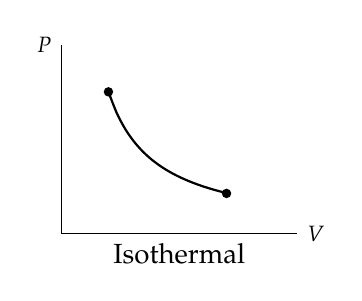
\begin{tikzpicture}[scale=.6]
      \draw(0,0)--(5,0) node[right]{\footnotesize $V$}
      node[midway,below]{Isothermal};
      \draw(0,0)--(0,4) node[left]{\footnotesize $P$};
      \draw[smooth,samples=15,domain=1:3.5,thick] plot({\x},{3/\x});
      \fill(1,3)   circle(.1);
      \fill(3.5,.85) circle(.1);
    \end{tikzpicture}
    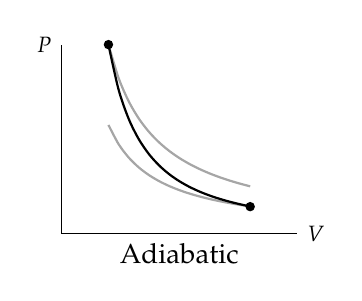
\begin{tikzpicture}[scale=.6]
      \draw(0,0)--(5,0) node[right]{\footnotesize $V$}
      node[midway,below]{Adiabatic};
      \draw(0,0)--(0,4) node[left]{\footnotesize $P$};
      \draw[smooth,samples=15,domain=1:4,thick,gray!70] plot({\x},{4/\x});
      \draw[smooth,samples=15,domain=1:4,thick,gray!70] plot({\x},{2.3/\x});
      \draw[smooth,samples=15,domain=1:4,thick] plot({\x},{4*((\x)^(-1.4))});
      \fill(1,4) circle(.1);
      \fill(4,.57) circle(.1);
    \end{tikzpicture}
  \end{center}
\end{frame}



\begin{frame}{A Simple Heat Engine Cycle}
  \begin{columns}
    \column{.8\textwidth}
    \pic{.5}{heat-engine}
    \begin{enumerate}
    \item\vspace{-.15in} Heat is added at constant volume; no work done.
    \item Heat is added as gas expands at constant pressure; work is done by
      the gas to lift the weight.
    \item Heat is extracted at constant volume; no work done.
    \item Heat is extracted at constant pressure; work is done on the gas to
      compress it.
    \end{enumerate}
    \column{.2\textwidth}
    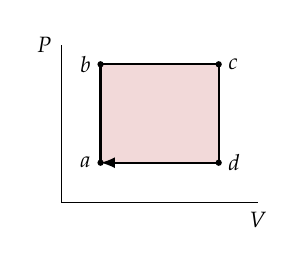
\begin{tikzpicture}[scale=.5]
      \fill[pink!80!gray!50](1,1) rectangle(4,3.5);
      \draw(0,0)--(5,0) node[below]{\footnotesize $V$};
      \draw(0,0)--(0,4) node[left]{\footnotesize $P$};
      \draw[thick,->](1,1)--(1,3.5)--(4,3.5)--(4,1)--(1,1);
      \fill(1,1) circle(.08) node[left]{\footnotesize$a$};
      \fill(1,3.5) circle(.08) node[left]{\footnotesize$b$};
      \fill(4,3.5) circle(.08) node[right]{\footnotesize$c$};
      \fill(4,1) circle(.08) node[right]{\footnotesize$d$};
    \end{tikzpicture}

    {\footnotesize $P$-$V$ diagram of the simple heat engine shown on the left.
      \par}
  \end{columns}
\end{frame}



\begin{frame}{Efficiency of Heat Engine}
  In a heat engine, the internal energy at the beginning and end of the cycle
  are the same (same point on the $P$-$V$ diagram), so the work done is just
  the difference between heat added and taken out:
  
  \eq{-.25in}{
    W = Q_\text{in}-Q_\text{out}
  }
  
  \vspace{-.15in}Efficiency is defined as the ratio between work done and heat
  added:

  \eq{-.25in}{
    \boxed{\eta =\frac{W}{Q_\text{in}}=1-\frac{Q_\text{out}}{Q_\text{in}}}
  }
\end{frame}


\begin{frame}{Second Law of Thermodynamics}
  \begin{block}{Kelvin-Planck Statement}
    It is impossible for heat engine working in a cycle to produce no other
    effect than that of extracting heat from a reservoir and performing an
    equivalent amount of work.
  \end{block}
\end{frame}



\begin{frame}{Carnot Engine}
  The Carnot engine cycle is the most efficient.
  \pic{.4}{carnot}
  The efficiency of a Carnot engine is:
  
  \eq{-.25in}{
    \boxed{\eta_C =1-\frac{Q_\text{out}}{Q_\text{in}}=1-\frac{T_c}{T_h}}
  }
\end{frame}
\end{document}
